\documentclass[conference]{IEEEtran}
\usepackage{cite}
\usepackage{amsmath,amssymb,amsfonts}
\usepackage{algorithmic}
\usepackage{graphicx}
\usepackage{textcomp}
\usepackage{xcolor}
\usepackage[numbers]{natbib}
\usepackage[normalem]{ulem}
\useunder{\uline}{\ul}{}

\def\BibTeX{{\rm B\kern-.05em{\sc i\kern-.025em b}\kern-.08em
    T\kern-.1667em\lower.7ex\hbox{E}\kern-.125emX}}

\begin{document}

\section*{Summary}
In this project, we are interested in doing time series forecasting using various machine and deep learning models.
The goal is to compare their performance when training on different datasets.
Time series forecasting concerns itself with predicting future behavior of some phenomenon based on existing historical data.
In our case, this would be predicting future temperatures based on existing historical data from different cities in the world.
We aim to create an application that allows a user to select a trained model for use in predicting the temperature of a  city at some specified timestamp.

\subsection{Why Machine Learning}
Historically, weather forecasting has always been an important part of day-to-day life, and recently machine and deep learning has gradually become a more common technique for this.
Popular methods include the application of models such as ARIMA, RNNs, LSTMs and GRUs.
Each of these models have limitations that make them problematic to use in time series forecasting, however.
For models such as RNNs, problems like the vanishing gradient limits its ability to learn over long time steps as the change of the internal weights will become miniscule, which, for long time steps, effectively prevents further training.
LSTMs and GRUs are improvements on RNN models, however they suffer from other issues such as the abundance of parameters that often lead to complex models that take a long time to train.

The primary model described and used in this project is the transformer model.
The transformer model has its origins in natural language processing (NLP) and was introduced in 2017 by \citet{AttentionIsAllYouNeed}. 
The aim of this model was to overcome some of the issues related to both the vanishing and exploding gradient problem as well as the performance issues seen in some models.
The primary component of this model is an attention mechanism called multi-head attention, which allows the model to do training in parallel and thus improve performance. 
The model is originally also comprised of an encoder layer and a decoder layer. 

\subsection{Our work}
In the paper, we describe a selection of models in detail and compare the performance of these.
Furthermore, we also detail the changes and additions made to the original architecture such that it can be used for time series forecasting.
Since the transformer model is indifferent to temporal information, we had to convert our input data into some vector representation containing both periodic and non-periodic information.
This was done following the approach presented in \citet{time2vec}.

Our application architecture consists of two primary components.
The first component is responsible for loading data and training the models.

Initially, the datasets, which are stored as CSV files, are loaded into a Jupyter notebook on Deepnote using the Python Pandas framework.
After this, the data are lagged with 10 timesteps - each timestep corresponds to a day.
This number is chosen based on the fact that the climate in the cities from the datasets is relatively stable, and therefore using 10 timesteps seemed reasonable when forecasting.
Then, the data are split into training and testing data, on which the given model is trained. 
Finally, the data and trained models are serialized as Python \texttt{pickle} files - a process known as pickling - which are then exported into the second the component; the web application.

The web application is structured as a normal client-server application.
When a client connects to the server, the web page is served to the client which contains the user interface for model selection.
The models are stored on the server and served to the client whenever the user selects a model through the dropdown menu on the web page.
Once the client receives the model, the resulting predictions are rendered as a graph on the web page.
The graph displays the model's predictions where the x-axis are the timesteps and the y-axis is the predicted feature values.

\subsection{Collaboration}
We used Deepnote\cite{deepnote} to train the models. 
The code for each model was contained in individual Python notebooks on Deepnote.
This allowed for easy collaboration between the group since Deepnote features a collaborative text editor.

The data we used are open source and downloaded from Kaggle\cite{kaggle}, and was provided by a variety of different contributors.
As such, it is worth noting that the data therefore came from arbitrary cities in the world, and that we are unable to verify its legitimacy.
This should be of no concern, however, since the primary goal was to use meaningfully large and representative datasets for training the models.


\subsection{Conclusion}
Having used weather data gathered from different weather sensors, we have trained and compared different machine learning models for time series forecasting.

The focus of this paper was to show that the transformer machine learning model would outperform previous state-of-the-art statistical and machine learning techniques. 
We have presented new evidence for this to be the case.
Additionally, we developed a web application to show the results of the trained models, and the user is able to interact with this web application by using a dropdown to select a model and a dataset. This will then show the temperature predictions.


\newpage

\title{Weather Forecasting}
\author{
    \IEEEauthorblockN{Christian B. B. Houmann}
    \and
    \IEEEauthorblockN{Daniel O. Nykjær}
    \and
    \IEEEauthorblockN{Ivik L. D. Hostrup}
    \and
    \IEEEauthorblockN{Patrick F. Østergaard}
}


\maketitle

\begin{abstract}
\input{sections/abstract.tex}
\end{abstract}

\begin{IEEEkeywords}
machine learning, weather forecasting
\end{IEEEkeywords}

\section{Introduction}
\section{Introduction}
\label{sec:intro}
A cyber-physical system (CPS) is a computerized system where real world physical events or mechanisms are monitored or controlled through the application of computer algorithms.
In a CPS, physical and software components work together in different spatial and temporal scales.

An example of such a system is how large weather sensor networks work in correlation. These produce both local weather time series, but they also affect how data from other sensors are interpreted. This, in turn, produces multiple weather time series that are all correlated. Being able to accurately forecast the weather has a large impact on most other CPSs as well as most people's daily lives. Having an accurate forecasting model is necessary in order to be able to accurately identify trends and outliers as well as predicting the future behavior of the weather. Ultimately all of this is useful in both the day to day running of other CPSs, and also in predicting future possible climate changes. 

To generate a reliable time series weather forecasting model, we need a model that is able to account for the seasonality aspect of the weather and the variable attributes that affect the future. 
This means that, in order to generate an accurate model, one must be able to take into account previous historical states when making predictions for the future. 

Today the state of the art methods in time series forecasting are methods such as autoregressive integrated moving average(ARIMA), Recurrent neural networks(RNN's), long short term memory(LSTM's) and gated neural networks(GRU's). Currently in the field of natural language processing (NLP) the transformer model[cite] is making large strides in improving the state of the art compared to the formerly used methods. Due to this we aim to measure the performance of a transformer modified to do univariate time series weather forecasting against the currently and formerly used methods. 



\section{Related Work}\label{sec:relatedwork}
\subsection{Statistical models}
For time series forecasting, a common approach is to use statistical analysis models like autoregressive integrated moving average (ARIMA).
ARIMA is a linear statistical analysis model that uses time series data to predict future trends.
It integrates two models.
The first model is the autoregression (AR) model, which is a model that forecasts a variable using a linear combination of past values of the same variable. 
The second model is the moving average model (MA), which instead of using past values, uses previously forecasted errors (residuals) to make current predictions. 
The final element in the ARIMA model, the I, is the differencing of observations in order to achieve stationarity, which is done to remove trends or seasonality that affect the value of the time series at different times. The primary drawback of the ARIMA model is the assumption of linearity in the time series data, which may, in fact, be non-linear.\cite{HybridArimaAndNN}\cite{ForecastinPrinciplesAndPractice}

\subsection{Machine learning}
Machine learning can also be used for time series forecasting. 
One such machine learning model is linear regression, which can be used to fit a linear function onto a set of data points.
In time series forecasting, it is used to fit a predictive model to a dataset of observed values over time.
By minimizing the error between the input and target values, linear regression generates the most accurately fitted linear function that estimates the prediction values.
Linear regression is highly explainable due to the semantics of how the model weighs the input features. 
In other words, if the weight of an input feature is negative, then it is inversely proportional to the output. \cite{pooleArtificialIntelligenceFoundations2017}

The primary the drawback of linear regression is the fact that is it assumes linearity between input and prediction values, which is rarely the case in the real world.
In addition, due to this linear assumption, linear regression is very sensitive to outliers as these greatly affect the resulting predictive model.
Therefore, predictions may be quite inaccurate in various practical applications. \cite{kumarProfessionalsPointAdvantages2019}
\subsection{Deep learning}
Another approach to time series forecasting is the use of neural networks.
\subsubsection{MLP models}
A Multilayer Perceptron consists of an input and output layer as well as one or more hidden layers. These hidden layers are made up of multiple neurons. 
Since MLPs are feedforward algorithms, the inputs are combined with an initial weight in a weighted sum and then passed to the activation function. 
Each of these hidden layers then feeds their output and their internal representation of the data to the next layer in the network until the output layer is reached.\cite{bentoMultilayerPerceptronExplained2021}

\subsubsection{RNN models}
A popular model is to use recurrent neural networks and derivations of this model. Recurrent neural networks are similar to feedforward networks, but have memory of the past which is achieved through a hidden state which is passed recurrently through from previous layer as input to the succeeding layer. This makes it capable of learning short patterns. 
A primary issue with RNNs are the vanishing gradient and the exploding gradient problem with longer patterns, which more powerful models seek to improve upon. \cite{AIModernApproach}\cite{hands-onML}

To combat the issues of the vanishing gradient and exploding gradient problem, the Long short-term memory (LSTM) model was introduced by Sepp Hochreiter et. al. The basic principle of this model is the ability to bridge time intervals across longer time steps, which is achieved through the maintenance, updating and filtering of information into a cell state, which propagates through the entire network\cite{LSTMPaper}. 
A more recent, simplified version of the LSTM model, is the gated recurrent network (GRU), proposed by Kyunghyun Cho et al. which merges the two state vectors in the LSTM into a single state vector, includes just a single gate controller that controls both the forget gate and the input gate and instead of an output gate which is present in the LSTM, the GRU outputs the entire state vector at every time step\cite{RNNPaper} \cite{hands-onML}.
Although LSTM and GRU models show significant improvements over regular RNN models in their ability to learn long term patterns, they are still inefficient at learning longer patterns as their inherent sequential nature can cause memory constraints\cite{AttentionIsAllYouNeed}. 

\section{Preliminaries}
\section{Preliminaries}
Given a cyber-physical system with \textit{N} sensors, each sensor is attributed with a time series.
Each timestamp in each of these time series contains information about \textit{C} features.
A time series of \textit{N} sensors can then be represented as \(X \in \mathbb{R}^{N \times C \times T}\).
The time series from the \textit{i}-th sensor is captured by \(x^{(i)} \in \mathbb{R}^{C \times T} \).
In addition, \(x_{t} \in \mathbb{R}^{N \times C}\) captures the time series of \textit{N} sensors at timestamp \textit{t} with \textit{C} features.
Finally, the vector of attributes for the \textit{i}-th sensor at timestamp \textit{t} is represented with \(x_{t}^{(i)} \in \mathbb{R}^{C}\).

\section{System Architecture}\label{sec:system architecture} % Methodology
As the purpose of the project is to create a system in which a user should be able to see the weather forecast for a specific area, or more precisely, the temperature forecast, we have developed a system that leverages several models to perform the temperature forecasting. 
The goal is to allow the user to interact with the system in such a way that the user can see the accuracy of the different models. 
On a web page, the user is able to select a city for which they want to predict the temperature. The results are shown both as a graph that displays the predicted value versus the actual value, as well as the specific set of temperatures of that city for a given time period into the future. This is similar to what one may see on regular weather forecasts.

In order to achieve, this we have constructed a pipeline that preprocesses the data, trains our models, and the resulting models are then used to perform the forecasting displayed on a web application. 
Figure \ref{fig:architecture diagram} shows an overview of the architecture of the pipeline.

Note that since the transformer model is the best performing model, which is shown in section \ref{sec:ExpRes}, this is the model that we chose to include and describe as part of the pipeline. Regardless of this fact, the other models are used in the pipeline in a similar fashion.

In section \ref{sec:data loading and preprocessing}, we start by presenting the data loading and preprocessing phase of the system architecture, and we also motivate our interest in the transformer model.
Then, in sections \ref{sec:self-attention mechanism} and \ref{sec:multi-head attention}, we describe preliminary theory about the transformer model; the self-attention mechanism and multi-head attention module. 
Afterwards, in section \ref{sec:time2vec} we introduce the method we use for embedding temporal information into the transformer model. 
In section \ref{sec:training}, we describe our approach to training the models, and how we serialize the formatted data and trained models into the Python \texttt{pickle} format.
Finally, in section \ref{sec:web app}, we introduce the front-end web application where the user is able to make predictions using our trained models using a simple graphical user interface in a web browser.



\begin{figure*}
	\centering
	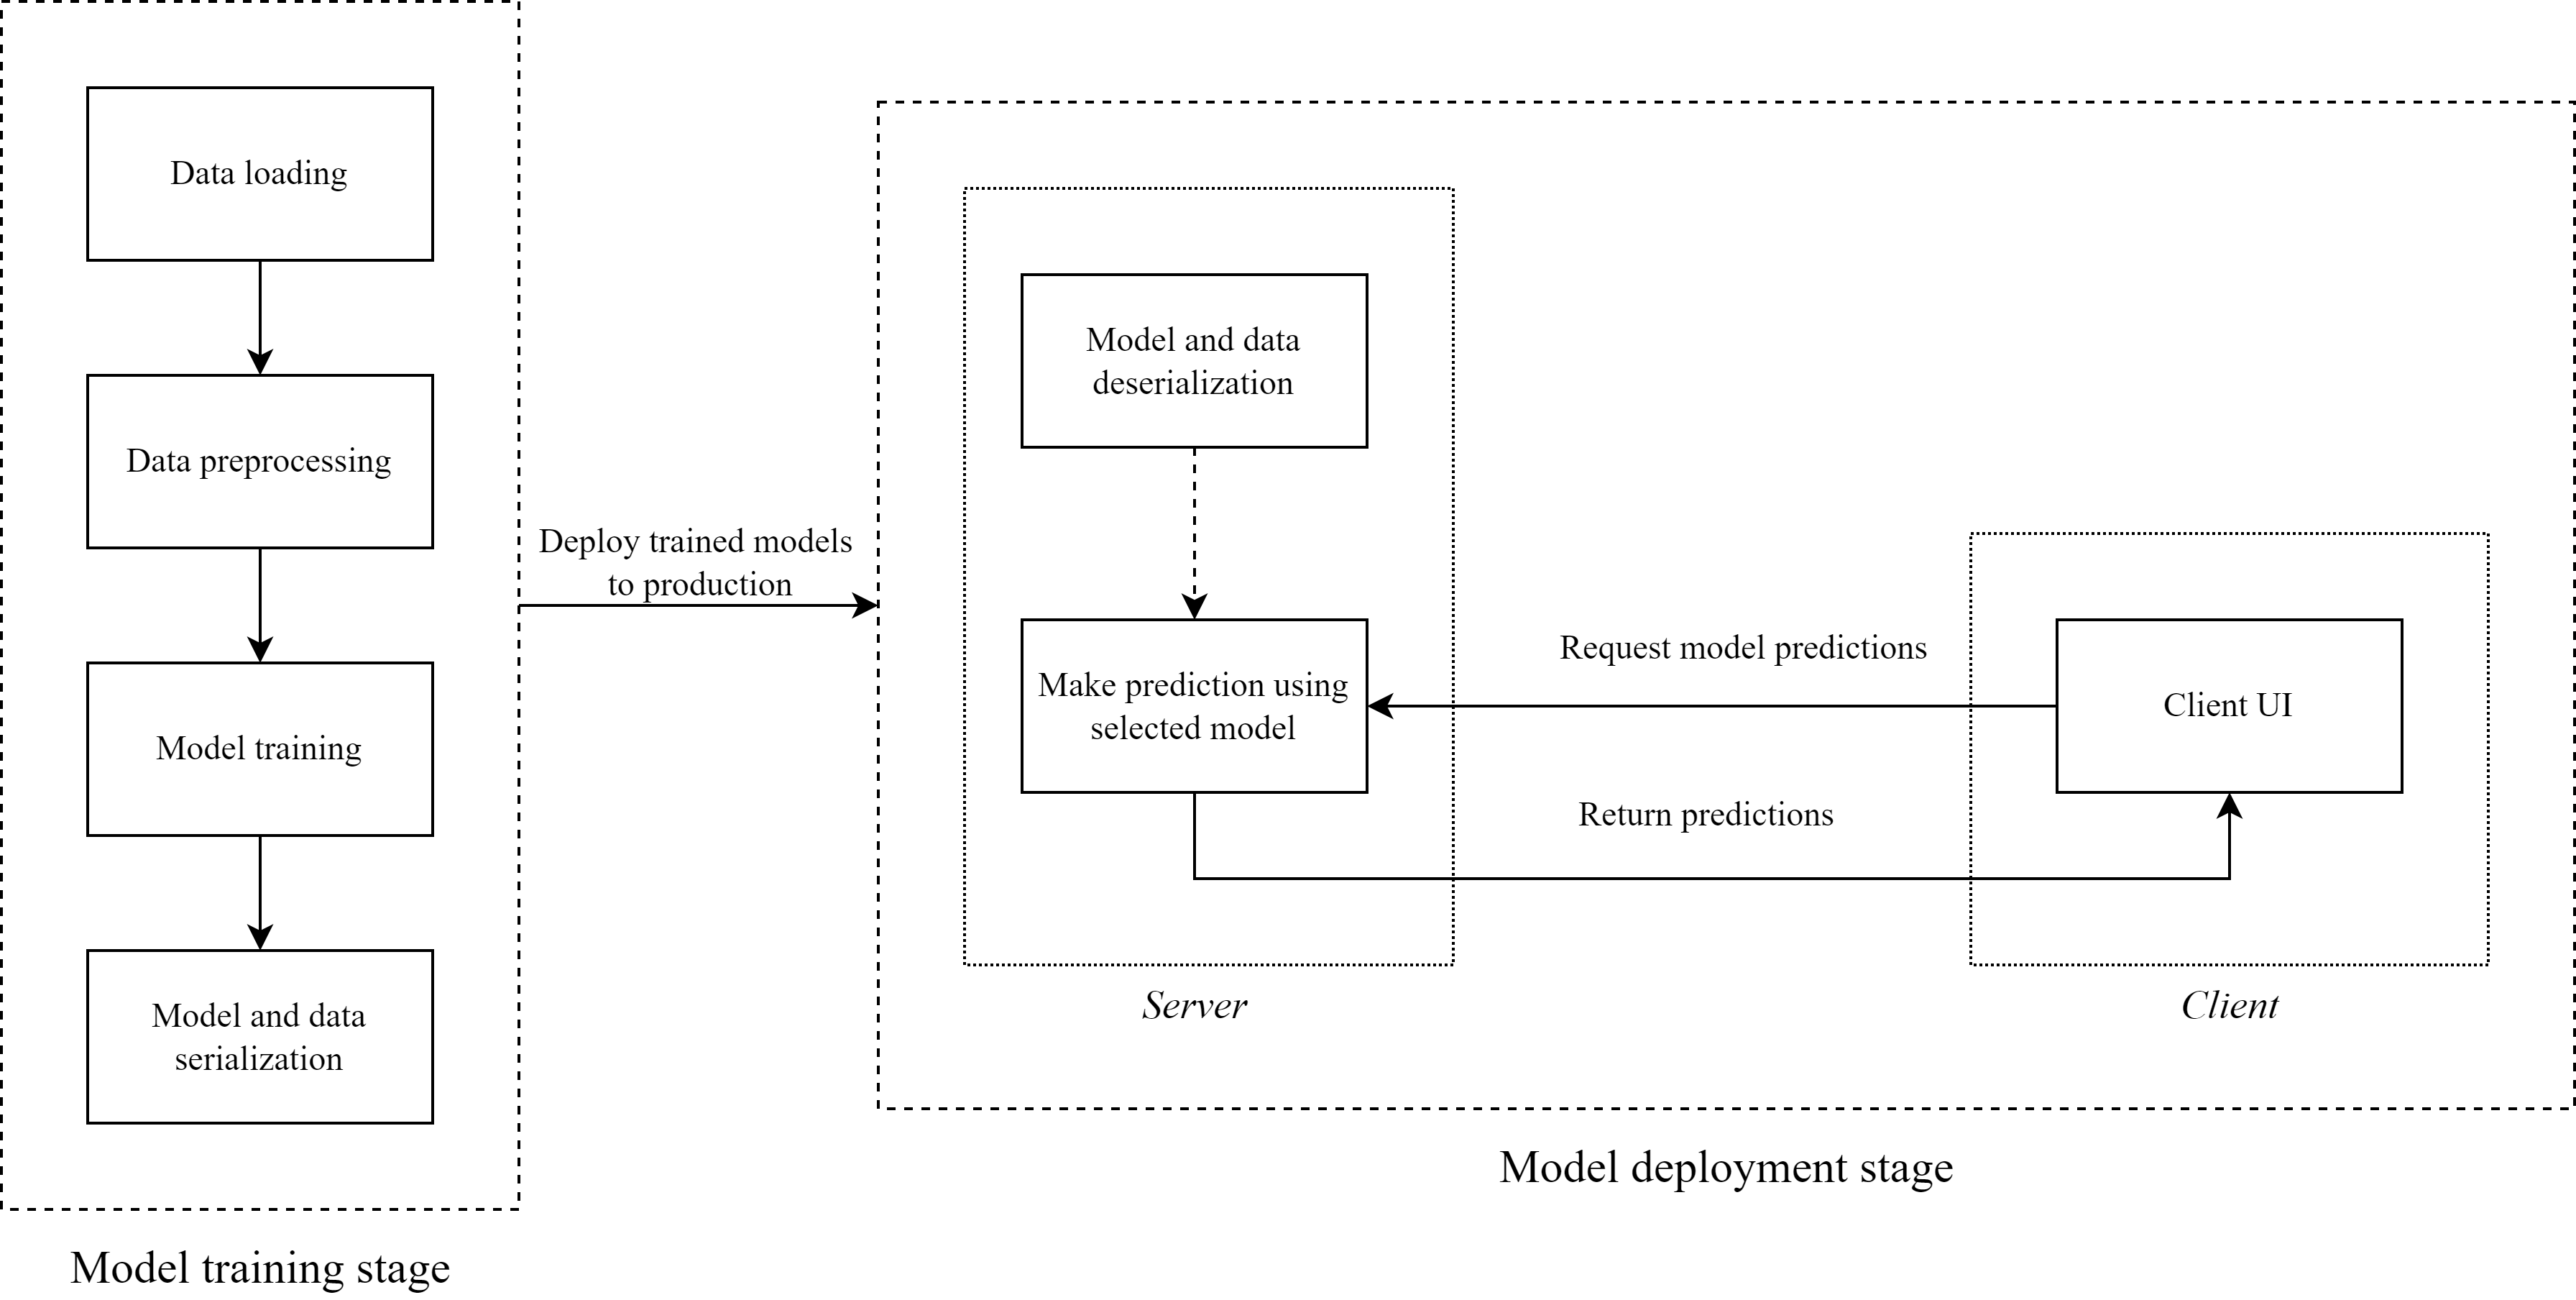
\includegraphics[width=1\textwidth]{Architecture diagram}
	\caption{The architecture of the system pipeline.}
	\label{fig:architecture diagram}
\end{figure*}
As the purpose of the project is to create a system in which a user should be able to see the weather forecast for a specific area, or more precisely, the temperature forecast, we have developed a system that leverages several models to perform the temperature forecasting. 
The goal is to allow the user to interact with the system in such a way that the user can see the accuracy of the different models. 
The user is able to select a region for which they want to predict the temperature. The results are shown both as a graph that displays the predicted value versus the actual value, as well as the specific set of temperatures of that region for a given time period into the future. This is similar to what one may see on regular weather forecasts.

In order to achieve, this we have constructed a pipeline that preprocesses the data, trains our models, and the resulting models are then used to perform the forecasting displayed on a web application. 
Figure xx shows an overview of the architecture of the pipeline.
Note that since the transformer model is the best performing model, which is shown in section (experiment afsnit), this is the model that we chose to include and describe as part of the pipeline. Regardless of this fact, the other models are used in the pipeline in a similar fashion.

\subsection{Data loading and preprocessing}
In order to load the data we have done the following...
\subsection{Self-attention Mechanism}\label{sec:self-attention mechanism}


With self-attention, the model can learn to associate different input.
To achieve this, three input vectors are needed - queries and keys of dimension $d_k$, and values of dimension $d_v$.
The attention function maps the query and the set of key-value pairs to some output, where the output is a weighted sum of the values.
The weight of each value is calculated using a compatibility function.
This weight denotes how compatible the query is with the given key.



The output matrix of weights is computed using the function
$$
Attention(Q, K, V) = softmax(\frac{QK^T}{\sqrt{d_k}})V
$$

Additive attention and dot product attention are among some of the most common attention functions used.
For the purposes of this project, we decided to use the scaled dot product attention technique with the scaling factor $\frac{1}{\sqrt{d_k}}$.
We use this technique as it is faster and more space-efficient as argued in \citet{AttentionIsAllYouNeed}.

Because the dot product can result in values between negative and positive infinity, the \textit{softmax} activation function is used to map values to the interval $[0,1]$, and to ensure that they sum to $1$ over the entire sequence. \cite{AttentionIsAllYouNeed}

\subsection{Multi-Head Attention}\label{sec:multi-head attention}
To improve the self-attention mechanism, the authors of the original transformer model implemented multi-head attention.
This is a module that runs through the previously described attention mechanism multiple times and in parallel.
It then concatenates the attention weights of all the independent self-attention layers. 

\begin{align*}
MultiHead(Q, K, V) = Concat(h_1, \ldots, h_i)W^O \\
\text{where }h_i = Attention(QW^Q_i, KW^K_i, VW^V_i) 
\end{align*}

In the model we use, the weights are then passed through a dense layer in which a non-linear transformation is applied using the \textit{ReLU} activation function rather than a linear transformation as described in \citet{AttentionIsAllYouNeed}. 
Once this computation is completed, the result is the final multi-head attention weight matrix. \cite{AttentionIsAllYouNeed}

\subsection{Time embedding}\label{sec:time2vec}
The transformer model is indifferent to temporal information.
Therefore, in order to embed our temporal data, we convert the input data to a vector representation.
Furthermore, vector representations are used for many different tasks, making a vector representation for time easily usable with a variety of different architectures.

To this end, we use the approach described in \citet{time2vec}. 
This paper conveys two main ideas.
Firstly, the time representation should contain both periodic and non-periodic information.
Secondly, the time representation should not be affected by different time increments and long time horizons.  

For a given scalar notion of time $\tau$, TimeToVector of $\tau$ is a vector of size $k + 1$ with the following definition:
$$
TimeToVector(\tau)[i] = 
\begin{cases}
  \omega_i \tau + \varphi_i, & \mbox{if $x<0$}.\\
  \mathcal{F}(\omega_i \tau + \varphi_i), & \mbox{if $1 \le i \le k$}.
\end{cases}
$$

where $TimeToVector(\tau)[i]$ is the \textit{i}th element of $TimeToVector(\tau)$, $\mathcal{F}$ is a periodic activation function (the sine function, in our case), and $\omega_i$ and $\varphi_i$ are learnable parameters. 

For $\mathcal{F} = sin, 1 \leq i \leq k$, $\omega_i$ is the frequency and $\varphi_i$ is the phase-shift.
Since the sine function is periodic, $\tau$ has the same value as $\tau + \frac{2\pi}{\omega_i}$, which helps capture periodic behavior without any feature engineering.
An example of this is the sine function $sin(\omega\tau + \varphi)$ with $\omega = \frac{2\pi}{7}$ can be used to model weekly patterns, assuming $\tau$ denotes days.
It is worth noting that the authors of the paper chose the sine function due to experiments showing that models using it outperform models that use non-periodic activation functions instead.\cite{time2vec}


\subsection{The transformer encoder layer}\label{sec:transformer encoder}
The previously described elements are now aggregated into a transformer encoder layer.
To improve the performance of the transformer, multiple of these layers can be stacked, and each of these encoder layers contain a self-attention sublayer as well as a feedforward sublayer. 

Once the multi-head attention weights have been computed, these weights are then fed into a dropout layer that has a residual connection consisting of the initial query.
Given some rate value, this layer randomly sets the input units to 0 using that rate as the frequency.
In other words, some values from the input are dropped, which helps prevent overfitting during training.

Following the dropout layer, the weights are normalized in a normalization layer. 
This gives us the final attention weights which are then passed to the feedforward layer.

The feedfoward layer is the dense layer, as described in section \ref{sec:multi-head attention}.
It should be noted that the two dense layers per encoder layer consist of 1-dimensional convoluted neural networks with a kernel size and stride of 1.
The output of these two layers are then fed into another dropout layer, which also has a residual connection consisting of the initial query. 

Finally, the values are normalized, which gives us the final transformer encoder output values.
The resulting architecture can be seen in figure \ref{fig:encoder transformer}.
As this figure demonstrates, the architecture is different from the original transformer architecture shown in \ref{fig:original transformer}.
Our transformer architecture is based on the architecture by \citet{schmitz_stock_2020}, which includes many of the original architectural elements from \textit{Attention Is All You Need} \cite{AttentionIsAllYouNeed}.
Because we are not working with natural language processing, there is no need for a decoder layer, since we do not to output any decoded data. 

\begin{figure}[h]
\centering
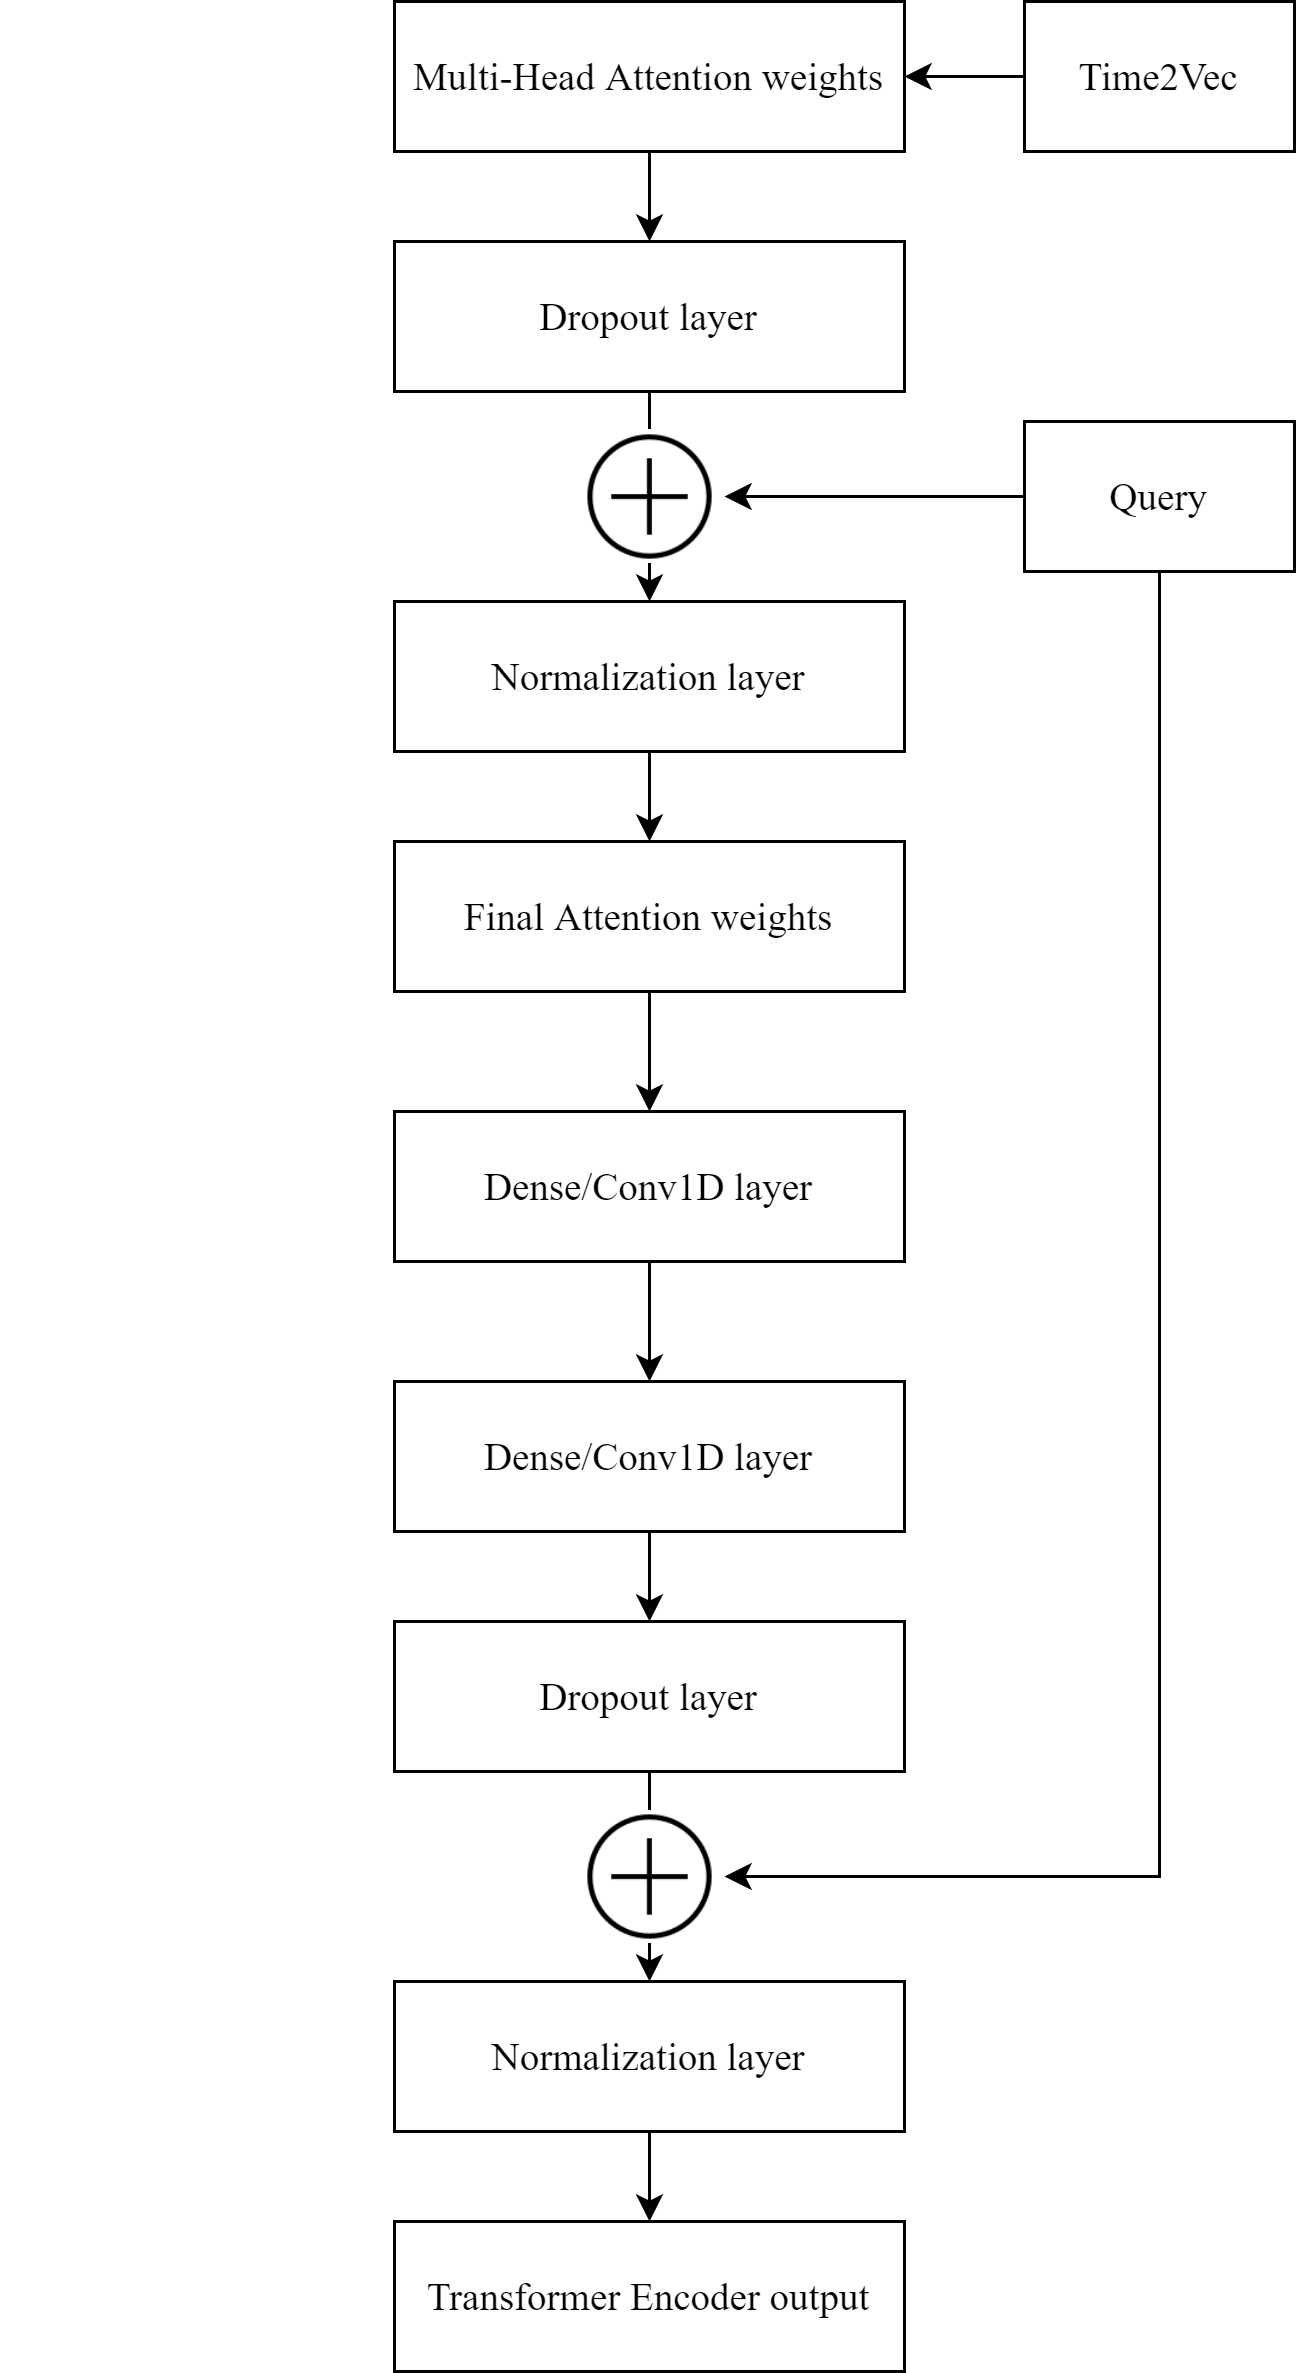
\includegraphics[width=0.375\textwidth]{Encoder transformer}
\caption{The transformer encoder layer.}
\label{fig:encoder transformer}
\end{figure}
\subsection{Training}\label{sec:training}
In order to train the models, we used Deepnote\cite{deepnote} to achieve similar hardware performance on the training of all the models used for this project. 
The training was done using individual Python notebooks contained in a project on Deepnote, in order to allow easy collaboration between the authors.

The data used are open source and was collected on Kaggle\cite{kaggle}. It was provided by individual contributors for free use.
The data came from arbitrary cities of the world. 
It should be noted that we cannot verify the legitimacy of the data, the main objective was simply to gather datasets that were representative and meaningfully large to train the models on. 
The training of each model used arbitrary settings for the batch sizes, hyperparameters, learning rates and dropout rates. Similarly, no optimization algorithms were implemented in order to identify the optimal settings. 

Once the models have been trained, they are serialized using the Python \texttt{pickle} module.
This module converts the data and the Python objects into a byte stream which is stored in a file.
The process of serializing Python objects is known as pickling. 
This allows us to export the trained models from Deepnote, the first component in our pipeline, and onto the server used in the web application, the second component in our pipeline, as previously shown in figure \ref{fig:architecture diagram}.\cite{pickle_documentation}
\subsection{Web application}
Once the models have been trained, 

\section{Experiments \& Analysis}\label{sec:ExpRes}
\begin{table*}[t]
    \centering
    \caption {Summary of gathered results---the best results are highlighted in bold and underlined.} \label{tab:ResultsTable} 
    \begin{tabular}{|l|r|r|r|r|r|}
    \hline
    \multicolumn{1}{|c|}{Models} & \multicolumn{1}{c|}{Austin} & \multicolumn{1}{c|}{Bangladesh} & \multicolumn{1}{c|}{Delhi} & \multicolumn{1}{c|}{Jena} & \multicolumn{1}{c|}{Szeged} \\ \hline
    ARIMA                        & 14.9971                     & 4.1595                          & 7.4077                     & 8.4354                    & 9.5993                      \\ \hline
    GRU                          & 12.1855                     & 3.6176                          & 3.8810                     & 3.5758                    & 5.0462                      \\ \hline
    LinReg                       & 13.465                      & 3.6610                          & 7.8551                     & 8.4248                    & 9.5464                      \\ \hline
    LSTM                         & 15.5649                     & 3.6178                          & 4.2537                     & 3.6141                    & 5.1415                      \\ \hline
    MLP                          & 15.3179                     & 3.7288                          & 7.5508                     & 8.6366                    & 10.6112                     \\ \hline
    RNN                          & 11.2289                     & 3.6152                          & 6.8748                     & 3.0483                    & 4.8869                      \\ \hline
    Transformer                  & {\ul{\textbf{7.4627}}}      & {\ul{\textbf{1.8536}}}          & {\ul{\textbf{2.4665}}}     & {\ul{\textbf{1.1787}}}    & {\ul{\textbf{2.0066}}}      \\ \hline
    \end{tabular}
\end{table*}

\begin{table*}[t]
    \centering
    \caption {Results normalized using standard deviation and sorted by lowest summed error in ascending order for each dataset.} \label{tab:ResultsTableSummed} 
    \begin{tabular}{|l|r|r|r|r|r|r|}
    \hline
        \multicolumn{1}{|c|}{Models} & \multicolumn{1}{c|}{Austin} & \multicolumn{1}{c|}{Bangladesh} & \multicolumn{1}{c|}{Delhi} & \multicolumn{1}{c|}{Jena} & \multicolumn{1}{c|}{Szeged} & \multicolumn{1}{c|}{Sum} \\ \hline
        Transformer & 0.4872 & 0.4971 & 0.3267 & 0.1365 & 0.1890 & {\ul{\textbf{1.6365}}} \\ \hline
        GRU & 0.7955 & 0.9702 & 0.5140 & 0.4140 & 0.4756 & {\ul{\textbf{3.1693}}} \\ \hline
        RNN & 0.7331 & 0.9695 & 0.9105 & 0.3530 & 0.4605 & {\ul{\textbf{3.4266}}} \\ \hline
        LSTM & 1.0161 & 0.9702 & 0.5633 & 0.4185 & 0.4845 & {\ul{\textbf{3.4527}}} \\ \hline
        LinReg & 0.8790 & 0.9818 & 1.0403 & 0.9755 & 0.8997 & {\ul{\textbf{4.7763}}} \\ \hline
        ARIMA & 0.9791 & 1.1155 & 0.9810 & 0.9767 & 0.9046 & {\ul{\textbf{4.9570}}} \\ \hline
        MLP & 1.0000 & 1.0000 & 1.0000 & 1.0000 & 1.0000 & {\ul{\textbf{5.0000}}} \\ \hline
    \end{tabular}
\end{table*}

In this section, we start by presenting the datasets used to conduct the experiments.
Afterwards, we list the baselines used in the experiments and describe general challenges involved in time series forecasting.
Finally, we present the results from the experiments and analyse them.

\subsection{Datasets}
The following datasets have been used when conducting experiments on the various machine learning algorithms used in this paper.
\begin{itemize}
    \item \textbf{Austin:} The raw dataset over weather features in Austin, Texas covers a 4 year period from 2013 to 2017 with data logged once per day in the period.
    \item \textbf{Bangladesh:} The weather dataset for Bangladesh was collected during the period 1901 to 2015 and shows the average monthly temperature during this period. 
    \item \textbf{Delhi:} The dataset covers weather data for Delhi, India from 2013 to 2017 with one day between each logged data point.
    \item \textbf{Szeged:} The raw dataset covers weather data for Szeged, Hungary from 2006 to 2016 generated every hour over a 10-year span.
    \item \textbf{Jena:} The dataset was recorded at the Max Planck Institute's weather station in Jena, Germany from 2009 to 2016.
\end{itemize}

\begin{table*}[!ht]
\centering
\caption {Dataset Statistics} \label{tab:DatasetTable}
\begin{tabular}{|l|r|r|ll}
\cline{1-3}
Dataset    & \multicolumn{1}{l|}{\#Samples} & \multicolumn{1}{l|}{\#Sample rate} &  &  \\ \cline{1-3}
Austin     & 1319                           & 1 Day                              &  &  \\ \cline{1-3}
Bangladesh & 1380                           & 1 Month                            &  &  \\ \cline{1-3}
Delhi      & 1578                           & 1 Day                              &  &  \\ \cline{1-3}
Jena       & 420451                         & 10 Minutes                         &  &  \\ \cline{1-3}
Szeged     & 96453                          & 1 Hour                             &  &  \\ \cline{1-3}
\end{tabular}
\end{table*}

We have used the root-mean-square-error (RMSE) as the loss function to compare the chosen machine learning algorithms. The formula for computing the RMSE can be seen below: 
$$RMSE = \sqrt{\frac 1 n \displaystyle\sum_{i=1}^n(Y_i - \hat{Y_i})^2}$$

\subsection{Baselines}

These models are taken from statistical, machine learning, and deep learning to get a better overview of how the transformer's results compare with other well-known models.
\begin{itemize}
    \item ARIMA\cite{ARIMA-book}: A generalisation of the ARMA model that can be fitted to data in order to predict future steps.
    \item GRU\cite{GRU-paper}: A RNN model similar to LSTM but with a forget-gate added instead of an output gate.
    \item LinReg: A standard linear regression model.
    \item LSTM\cite{LSTM-paper}: A model modifying the RNN memory system in order to combat the common vanishing gradient problem.
    \item MLP\cite{MLP-paper}: The classic neural network used for regression prediction problems.
    \item RNN\cite{RNN-paper}: The standard recurrent neural network model.
    \item Transformer\cite{AttentionIsAllYouNeed}: A state of art model used in NLP, modified to work for time series forecasting.
\end{itemize}

\subsection{Results}\label{sec:results}
Table \ref{tab:ResultsTable} summarizes the best performances of the tested models for each of the five datasets used. 
As can be seen, the transformer performs the best in all datasets. The reason for this is two-fold. 
The first reason is the time embedding component in the transformer, which allows the transformer to account for both periodic and non-periodic data and thus account for seasonality in the data. 
The second reason is the multi-head attention mechanism which, combined with the time embedding, allows the transformer to account for long-term dependencies. Models such as ARIMA can account for seasonality but struggles with long-term dependencies. 

RNNs are able to account for seasonality, but as described in section \ref{subsec:RNNModels}, they are expected to falter with long time steps due to the vanishing and exploding gradient problem. Table \ref{tab:ResultsTable} does, however, show that RNN performs well on all datasets except for the Delhi dataset. This issue may be related to the structure of the data or tuning of the hyperparameters, but analysis of this issue is out of scope for the paper.

LSTMs and GRUs can also account for seasonality but are expected to perform better with long time steps than RNNs. 
However, the LSTM model in our experiment is outperformed by the RNN model on all datasets except for the Delhi dataset.
We expected LSTM to perform similarly to GRU and consequently, we expected it to outperform the RNN model.

Linear regression and MLP are behaving as expected.

Standard deviation normalization was performed to account for the variability in the temperature depending on the region of the world in which the temperature data is captured. 
For example, data captured close to the equator may be higher and therefore the RMSE is also amplified in equal proportion. 
In order to compute the values seen in table \ref{tab:ResultsTableSummed}, the model errors from table \ref{tab:ResultsTable} were divided by the standard deviation calculated for each dataset.
The sum column shows the overall performance for each model, where the lowest number represents the best-performing model. 

\section{Conclusion}
Using weather data gathered from different cyber physical systems in the form of weather sensors, we have trained and compared several different techniques for time series forecasting.
Our main focus was to show that the transformer would outperform previous state-of-the-art statistical and machine learning techniques.
As can be seen in the \nameref{sec:ExpRes} section, the transformer indeed has the lowest RMSE error compared to the other models on every dataset. 
It is worth noting that the transformer used here deviates slightly from the original transformer model proposed by \citet{AttentionIsAllYouNeed}, as we have removed the decoder and implemented the time embedding module presented by \citet{time2vec}.
These are described in detail in section \ref{sec:system architecture}.

We have developed a web application to show the predictions from all the trained models in a simple graphical user interface. 
The user of the application is able to make temperature predictions by selecting a model and dataset from a dropdown menu. 

In the future, it would be interesting to study the reason for the RNN outperforming the LSTM model.
Based on the \nameref{sec:relatedwork} section, we expected the LSTM model to outperform the RNN model on these larger datasets.
One could run these on more and larger datasets to investigate whether this is still the case. 
In addition, it could also be beneficial to experiment further with hyperparameter tuning for all models.

In the future it would also be beneficial to update the web application to retrain the models daily with new weather data. It would also be beneficial to update the models to do multivariate forecasting.

In conclusion, the results from our experiments present new evidence suggesting that the transformer is better suited for time series forecasting than previous state-of-the-art techniques.

%\section*{Acknowledgment}

\bibliographystyle{IEEEtranN}
\bibliography{bib/bib}

\appendix
%\input{appendix/...}

\end{document}